\chapter{PJ3}



\section{記分板}

\subsection{次代記分板}
\begin{figure}[h]
  \centering
  \subfigure[次代記分板-1]{
    \includegraphics[width=0.3\textwidth]{timer1.png}
    \label{fig:image1}
  }
  \hfill
  \subfigure[次代記分板-2]{
    \includegraphics[width=0.3\textwidth]{timer2.png}
    \label{fig:image2}
  }
  \hfill
  \subfigure[次代記分板-3]{
    \includegraphics[width=0.3\textwidth]{timer3.png}
    \label{fig:image3}
  }
  \hfill
  \subfigure[次代記分板-4]{
    \includegraphics[width=0.3\textwidth]{timer4.png}
    \label{fig:image3}
  }
  \hfill
  \subfigure[次代記分板-5]{
    \includegraphics[width=0.3\textwidth]{timer1.0-1.png}
    \label{fig:image3}
  }
  \hfill
  \subfigure[次代記分板-6]{
    \includegraphics[width=0.3\textwidth]{timer1.0-3.png}
    \label{fig:image3}
  }
  \hfill
  \subfigure[次代記分板-7]{
    \includegraphics[width=0.3\textwidth]{timer1.0-5.png}
    \label{fig:image3}
  }
  \hfill
  \subfigure[次代記分板-8]{
    \includegraphics[width=0.3\textwidth]{timer1.0-4.png}
    \label{fig:image3}
  }
  \hfill
  \subfigure[次代記分板-9]{
    \includegraphics[width=0.3\textwidth]{timer1.0-2.png}
    \label{fig:image3}
  }
  \caption{次代記分板設計圖}
  \label{fig:multi_images}
\end{figure}


\newpage
\subsection{三代記分板}

\begin{flushleft}
\fontsize{14pt}{20pt}\sectionef\hspace{12pt}\quad 三代的數字都改模成新版的個別分件,通過平面配合各自組裝,使其可更加明顯,且外殼多擴兩孔、齒輪微調和增加輔助軸,使輪盤更方便抓到支點且連動更順滑,雖然變化看起來不大但總體表現都有一定更新
\end{flushleft}

\begin{figure}[h]
  \centering
  \subfigure[三代記分板-1]{
    \includegraphics[width=0.3\textwidth]{timer10.png}
    \label{fig:image1}
  }
  \hfill
  \subfigure[三代記分板-2]{
    \includegraphics[width=0.3\textwidth]{timer9.png}
    \label{fig:image2}
  }
  \hfill
  \subfigure[三代記分板-3]{
    \includegraphics[width=0.3\textwidth]{timer5.png}
    \label{fig:image3}
  }
  \hfill
  \subfigure[三代記分板-4]{
    \includegraphics[width=0.3\textwidth]{timer6.png}
    \label{fig:image3}
  }
  \hfill
  \subfigure[三代記分板-5]{
    \includegraphics[width=0.3\textwidth]{timer2.0-1.png}
    \label{fig:image3}
  }
  \hfill
  \subfigure[三代記分板-6]{
    \includegraphics[width=0.3\textwidth]{timer2.0-3.png}
    \label{fig:image3}
  }
  \hfill
  \subfigure[三代記分板-7]{
    \includegraphics[width=0.3\textwidth]{timer2.0-5.png}
    \label{fig:image3}
  }
  \hfill
  \subfigure[三代記分板-8]{
    \includegraphics[width=0.3\textwidth]{timer2.0-4.png}
    \label{fig:image3}
  }
  \hfill
  \subfigure[三代記分板-9]{
    \includegraphics[width=0.3\textwidth]{timer2.0-2.png}
    \label{fig:image3}
  }
  \caption{三代記分板設計圖}
  \label{fig:multi_images}
\end{figure}









\newpage
\section{球員}

\subsection{666系列:}
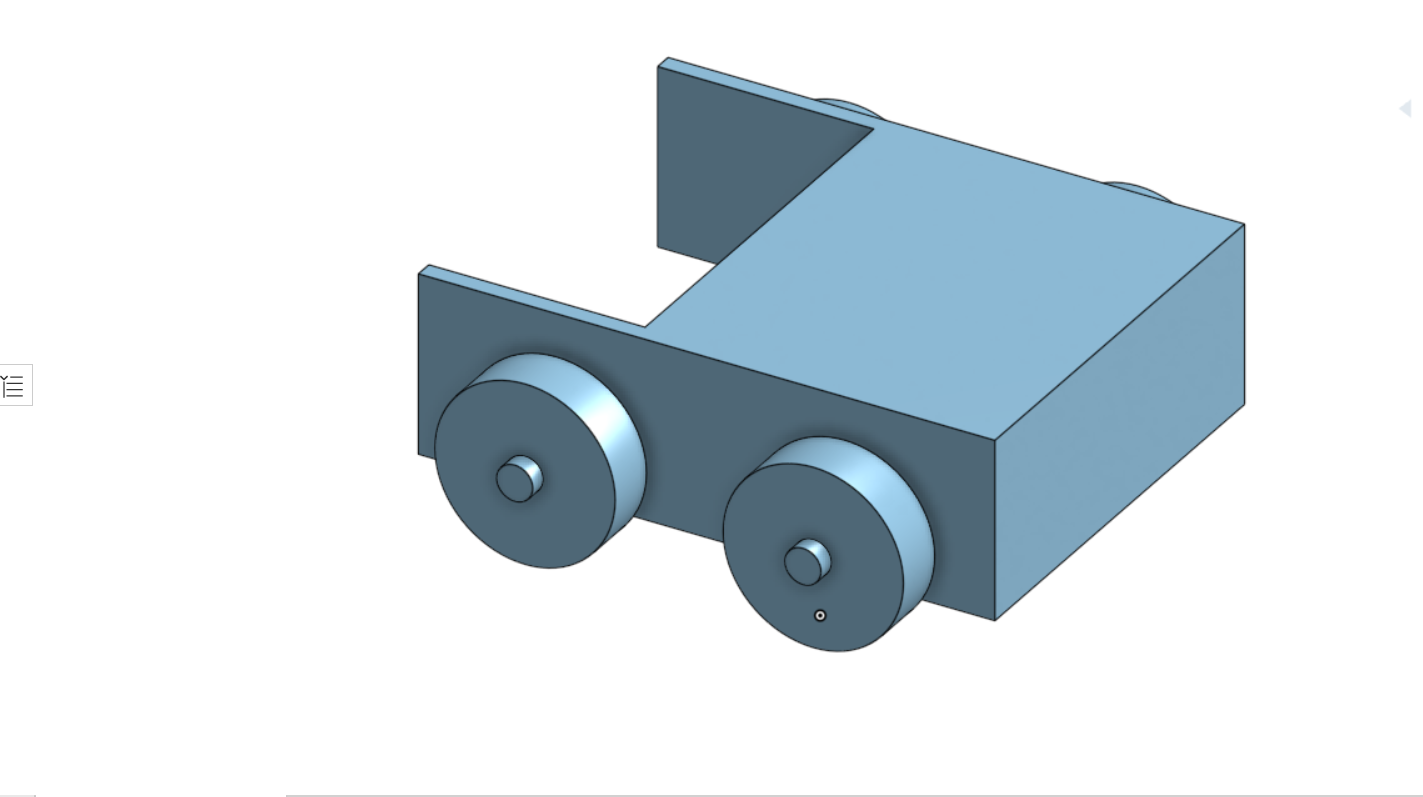
\includegraphics[width=0.5\textwidth]{robot-110系列.png}
\subsection{robot-00系列:}
\subsection{Maskie Razzio系列:}